\documentclass{article}
\usepackage[margin=1.5cm,bottom=2cm]{geometry}
\usepackage{fancyhdr}
\usepackage{graphicx}
\usepackage{amsmath}
\usepackage[section]{placeins}
\pagestyle{fancy}

\begin{document}
\fancyhead[L]{ 
\includegraphics[width=2cm]{au_logo.png} }
\fancyhead[R]{PHYS 2250: General Physics II}
\fancyfoot[C]{\thepage}
\vspace*{0cm}
\begin{center}
	{\LARGE \textbf{Lab 5}}\\
	\vspace{.5cm}
	{\Large RC Circuits: Charging and Discharging}
	%\vspace{0.25cm}
	%{\Large Due: Friday, September 4}
\end{center}

\section*{Introduction}
In class, we discussed the mechanisms driving the charging and discharging of a capacitor in a circuit with both a resistor and a capacitor (usually called an ``$RC$'' circuit ). In each case, current decreases at an ever slower rate until it eventually reaches 0. The question remains: what determines how quickly this happens? In this lab, you will track the time necessary for current to drop for different types of capacitors and resistors.

\section*{Procedure}
You will build both $RC$ charging and discharging circuits for several different combinations of resistors and capacitors. For each circuit you will measure the decay time of the current (instructions below) and record your data in a table (see Figure \ref{tab}. Make two tables, one for charging time, one for discharging time.

\begin{figure}[ht!]
	\centering
	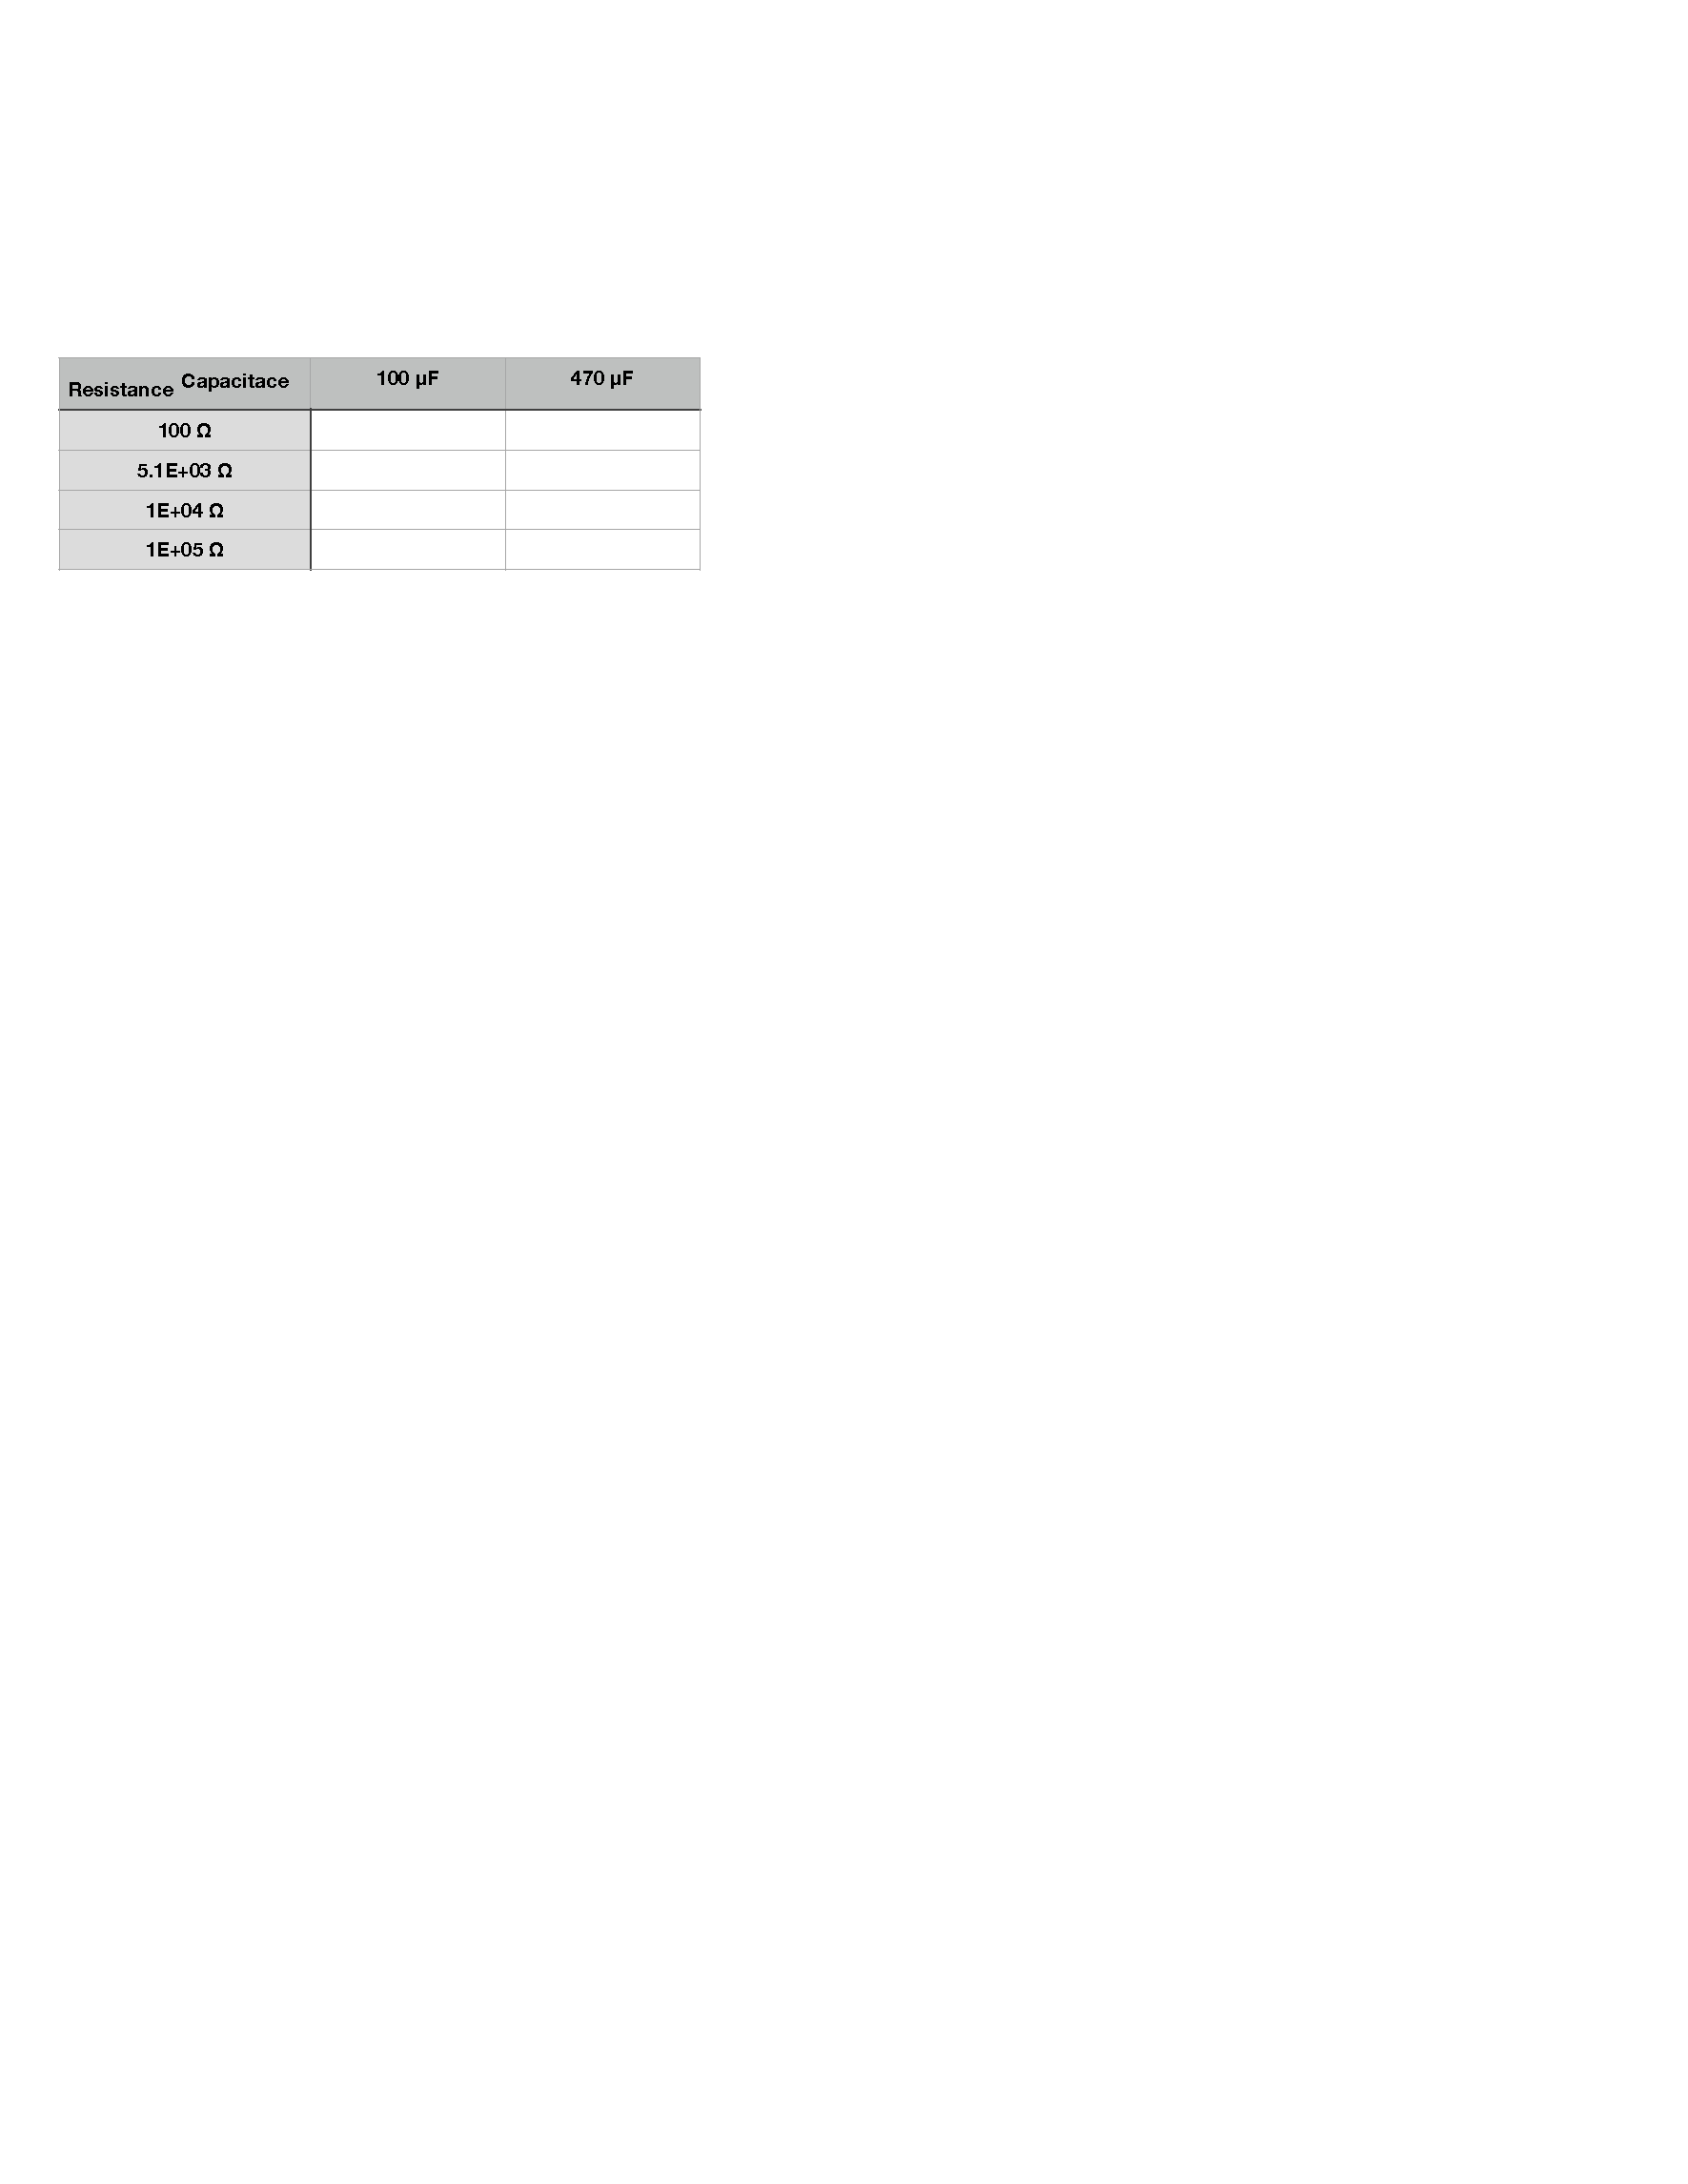
\includegraphics[width=10cm]{rc_table}
	\caption{An example data table}
	\label{tab}
\end{figure}

\begin{enumerate}
	\item Set up your charging circuit (Figure \ref{charging}). \textbf{Do not connect the circuit yet!}
	
	\begin{figure}[ht!]
		\centering
		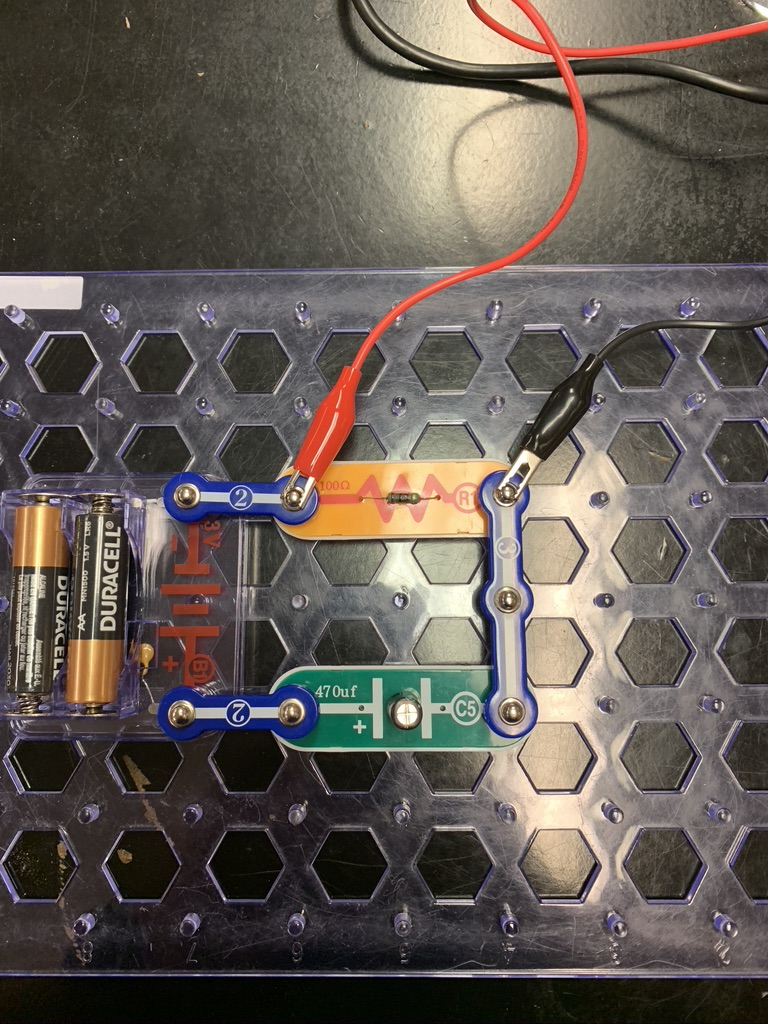
\includegraphics[width=5cm]{rc_charge.jpeg}
		\caption{A charging circuit, with voltage measured across the resistor}
		\label{charging}
	\end{figure}
	
	\item Set up the voltmeter to measure potential difference across the resistor.
	\item Start data collection, and then connect the circuit
	\item In LoggerPro: select the portion of the graph corresponding to your data, and then press the ``Curve Fit'' in the menu at the top of the screen. Choose "natural exponent" ($A*\exp(-C*t) + B$), then ``Try Fit''. The time value you want is $1/C$.
	\item Save an image of at least one graph for every capacitor you use (total of two graphs).
	\item Now disconnect the battery and create a discharging circuit like the one shown in figure \ref{discharging}. \textbf{Do not connect the circuit until you have begun data collection}. Repeat steps 2-5 for the discharging circuit: record and fit the data, find the time value $1/C$.
	
	\begin{figure}[ht!]
		\centering
		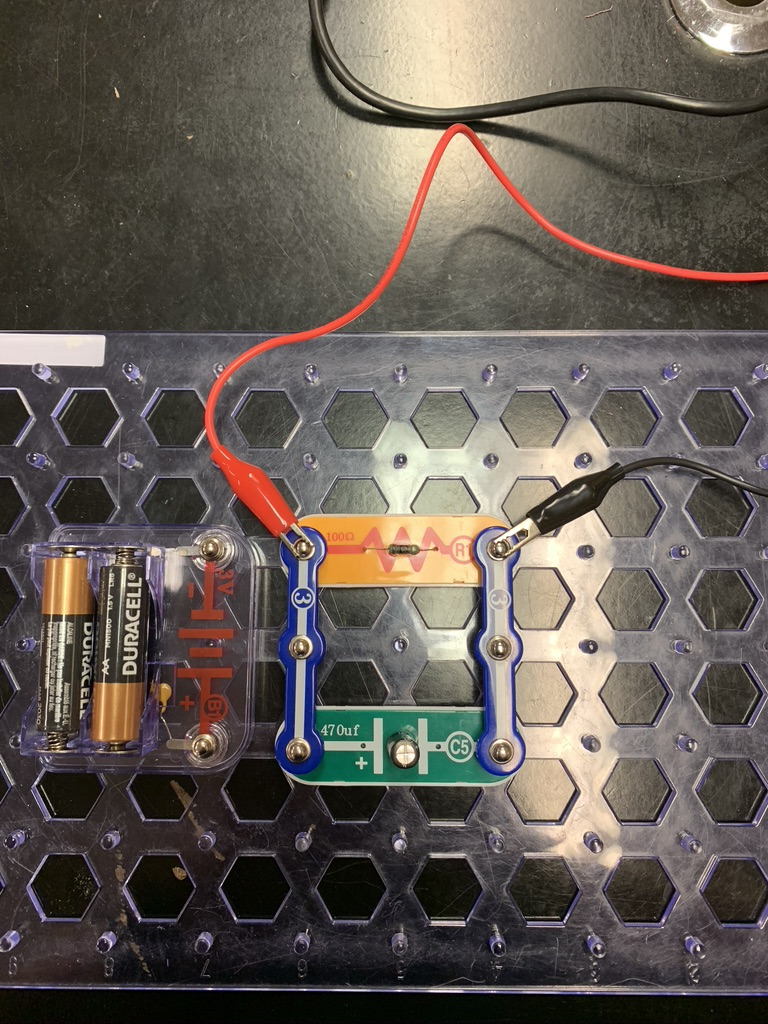
\includegraphics[width=5cm]{rc_discharge.jpeg}
		\caption{A discharging circuit}
		\label{discharging}
	\end{figure}
\end{enumerate}

\section*{Analysis}
\begin{enumerate}
	\item For both capacitors, make a graph of your time measurement vs resistance. How does increasing the resistance affect the charging/discharging time of the capacitor?
	\item What is the effect of increasing the capacitance of the capacitor on the charging/discharging time?
	\item How does the charging time of the capacitor compare to the discharging time?
\end{enumerate}
\end{document}